% ~ 6 pages
\chapter{Machine Learning}
\label{sec:ml}

\begin{itemize}
\item Supervised learning
\item Classification
\item Over-fitting
\end{itemize}

\section{Boosted Decision Trees}
\label{sec:bdt}

Keep this short!

Elements of statistical learning \cite{esl}

\begin{itemize}
\item Boosting: Adaptive Boosting $\alpha$, Gradient Boosting $\eta$
\item Node splitting: Gini Index
\item Hyperparameters: $N_\mathrm{Trees}$, $d_\mathrm{Tree}$,
\end{itemize}

\section{Neural Networks}
\label{sec:nn}

\subsection{Basics}
\label{sec:nn_basics}

Perceptron:
\begin{align*}
  y = \varphi(W x + b)
\end{align*}

Multi-layer perceptron (1 hidden layer):
\begin{align*}
  y &= \varphi_y(W_{yh} h + b_y) \\
  h &= \varphi_h(W_{hx} x + b_h)
\end{align*}

Layers are connected via linear transformations $W$ (and optionally
biases $b$) followed by a non-linear activation function $\varphi$.
Typical activation functions are:
\begin{align*}
  &\varphi(x) = \frac{1}{1 + e^{-x}} &\text{Logistic / Sigmoid Function} \\
  &\varphi(x) = \tanh(x) &\text{Hyperbolic Tangent} \\
  &\varphi(x) = \max(0, x) &\text{ReLU: Rectified Linear Unit} \\
  &\varphi(x) = &\text{Softmax}
\end{align*}

Forward pass:
\begin{itemize}
\item Forward pass (Feedforward Neural Networks)
\item Densely connected layers
\item Activation
\end{itemize}
Training:
\begin{itemize}
\item Weight initialisation
\item Loss functions
\item Mini-batch Gradient Descent
\item Cross-Validation
\end{itemize}

Logistic function:
\begin{align*}
  S(x) = \frac{1}{1 + e^{-x}}
\end{align*}

\begin{align*}
  \varphi(x) = \max(0, x) \quad \text{(ReLU)} \qquad \varphi(x) = \tanh(x)
\end{align*}

Loss for entry $i$. $j$ marks the class.
\begin{align*}
  L_i^\mathrm{binary} &= -t_i \log(p_i) - (1 - t_i) \log(1 - p_i) \\
  L_i^\mathrm{categorical} &= - \sum_j t_{ij} \log(p_{ij}) \\
  L &= \frac{\sum_i w_i L_i}{\sum_j w_j}
\end{align*}
Binary cross entropy follows from categorical cross entropy if
$p_{i1} + p_{i2} = 1$ and $t_{i1} + t_{i2} = 1$ for all $i$. Typical for
classification (e.g.\ using softmax) $\sum_i p_i = 1$ and $\sum_i t_i = 1$.
Motivate where in this thesis these loss functions are used.

\section{Recurrent Neural Networks}
\label{sec:rnn}

Recurrent: If a network has one or more cycles, that is, if it is possible to
follow a path from a unit back to itself.

Physics motivation: Able to do regression and classification on sequences of
physics objects like tracks, clusters, particle flow objects etc..

\subsection{Fully-Connected RNN}
\label{sec:fully_connected_rnn}

\textsc{Elman} network [Check Citation]\cite{elman}:
\begin{align*}
  c_t &= \sigma_c(W_c x_t + U_c c_{t-1} + b_c) \\
  h_t &= \sigma_h(W_h c_t + b_h)
\end{align*}

Elman or Jordan network?

Vanishing gradient problem: Applying the sigmoid function multiple times leads
to vanishing gradients (plot?).

\subsection{Long Short-Term Memory}
\label{sec:lstm}

\begin{figure}[t]
  \centering
  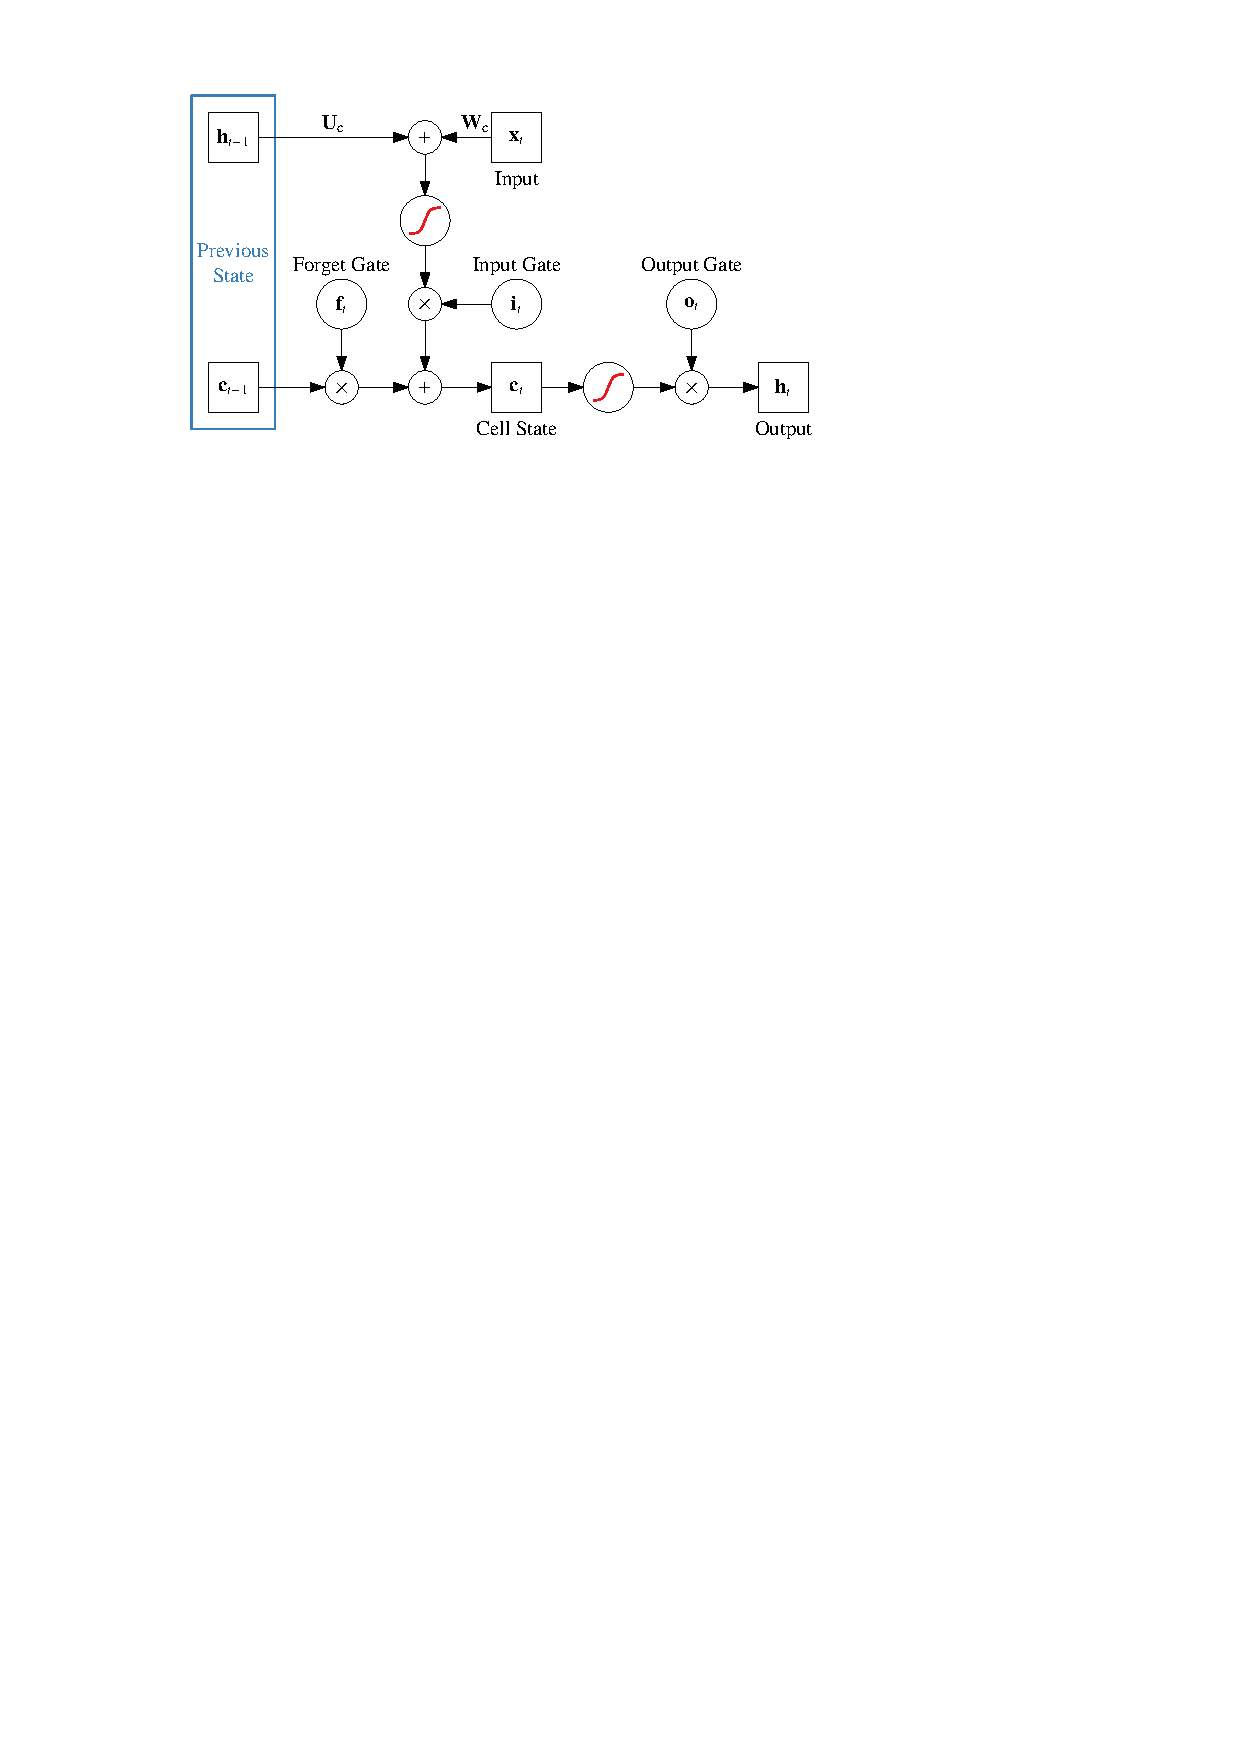
\includegraphics{./figures/theory/LSTM.pdf}
  \caption{Schematic description of a LSTM-cell.}
  \label{fig:schematic_lstm}
\end{figure}

[Check Citation]\cite{lstm}
\begin{align*}
  f_t &= \sigma_g( W_f x_t + U_f h_{t-1} + b_f) \\
  i_t &= \sigma_g( W_i x_t + U_i h_{t-1} + b_i) \\
  o_t &= \sigma_g( W_o x_t + U_o h_{t-1} + b_o) \\
  c_t &= f_t \circ c_{t-1} + i_t \circ \sigma_c(W_c x_t + U_c h_{t-1} + b_c) \\
  h_t &= o_t \circ \sigma_h(c_t)
\end{align*}

Stress that the gates depend on $x_t$ and $h_{t-1}$ via learn-able weights.
Therefore the inputting, outputting and forgetting is a learned process.

$\circ$: entry-wise product


Variables:
\begin{itemize}
\item $x_t$: input vector
\item $h_t$: output vector
\item $c_t$: cell state vector
\item $W$, $U$ and $b$: (recurrent -- $U$) weight matrices and bias vector
\item $f_t$, $i_t$ and $o_t$: gate vectors
  \begin{itemize}
  \item $f_t$: forget gate vector
  \item $i_t$: input gate vector
  \item $o_t$: output gate vector
  \end{itemize}
\end{itemize}

Activation functions:
\begin{itemize}
\item $\sigma_g$: element-wise sigmoid function (Gate activation -- recurrent
  activation)
\item $\sigma_c$: element-wise hyperbolic tangent (Cell activation -- recurrent
  activation)
\item $\sigma_h$: element-wise hyperbolic tangent (Output activation)
\end{itemize}


\section{Technical Setup}
\label{sec:tech_setup}

Frameworks used for this thesis (theano \cite{theano}, keras \cite{keras})

Optimiser: Adam

Masking layer


%%% Local Variables:
%%% mode: latex
%%% TeX-master: "mythesis"
%%% End:
